\documentclass{beamer}

\mode<presentation>
{
%\usetheme{Warsaw} %ok
%\usetheme{Rochester}
%\usetheme{Madrid}
%\usetheme{Pittsburgh}
%\usetheme{Antibes}
%\usetheme{Montpellier}
%\usetheme{Berkeley}
%\usetheme{PaloAlto}
%\usetheme{Goettingen}
%\usetheme{Marburg}
%\usetheme{Hannover}
%\usetheme{Berlin}
%\usetheme{Ilmenau}
%\usetheme{Dresden}
%\usetheme{Darmstadt}
\usetheme{Frankfurt} %ok
%\usetheme{Singapore} %ok
%\usetheme{Szeged}
%\usetheme{Copenhagen} %ok
%\usetheme{Malmoe}
\setbeamercovered{transparent}
}
% Choose color scheme
%
%\usecolortheme{default}
%\usecolortheme{sidebartab}
%\usecolortheme{albatross}
%\usecolortheme{beetle} 
%\usecolortheme{crane}
%\usecolortheme{dove} 
%\usecolortheme{fly} 
%\usecolortheme{seagull}
%\usecolortheme{lily}
\usecolortheme{orchid}
%
\usepackage{graphicx}
\usepackage[english]{babel}
\usepackage[utf8]{inputenc}

\def\etal{\emph{et al}.}
\def\v#1{\protect\vec #1}

%==============================================================================

\title{Recognizing human actions in still images:
a study of bag-of-features and part-based
representations}
\author{Vincent Delaitre, Ivan Laptev and Josef Sivic}

\begin{document}

\maketitle

%==============================================================================
\begin{frame}
\tableofcontents
\end{frame}

%==============================================================================
\section{Introducing a new dataset}
\begin{frame}
\frametitle{Introducing a new dataset}
We collected a new challenging dataset for real-life human actions. 

It is composed of 968 images collected from Flickr representing natural variations in terms of 
camera view-point, human pose, clothing, occlusions and scene background.

Pictures are distributed among 7 different classes: 
\begin{itemize}
\item Interacting with a computer
\item Taking a photograph
\item Playing music
\item Riding bike
\item Riding horse
\item Running
\item Walking
\end{itemize}

\end{frame}

%------------------------------------------------------------------------------

\begin{frame}
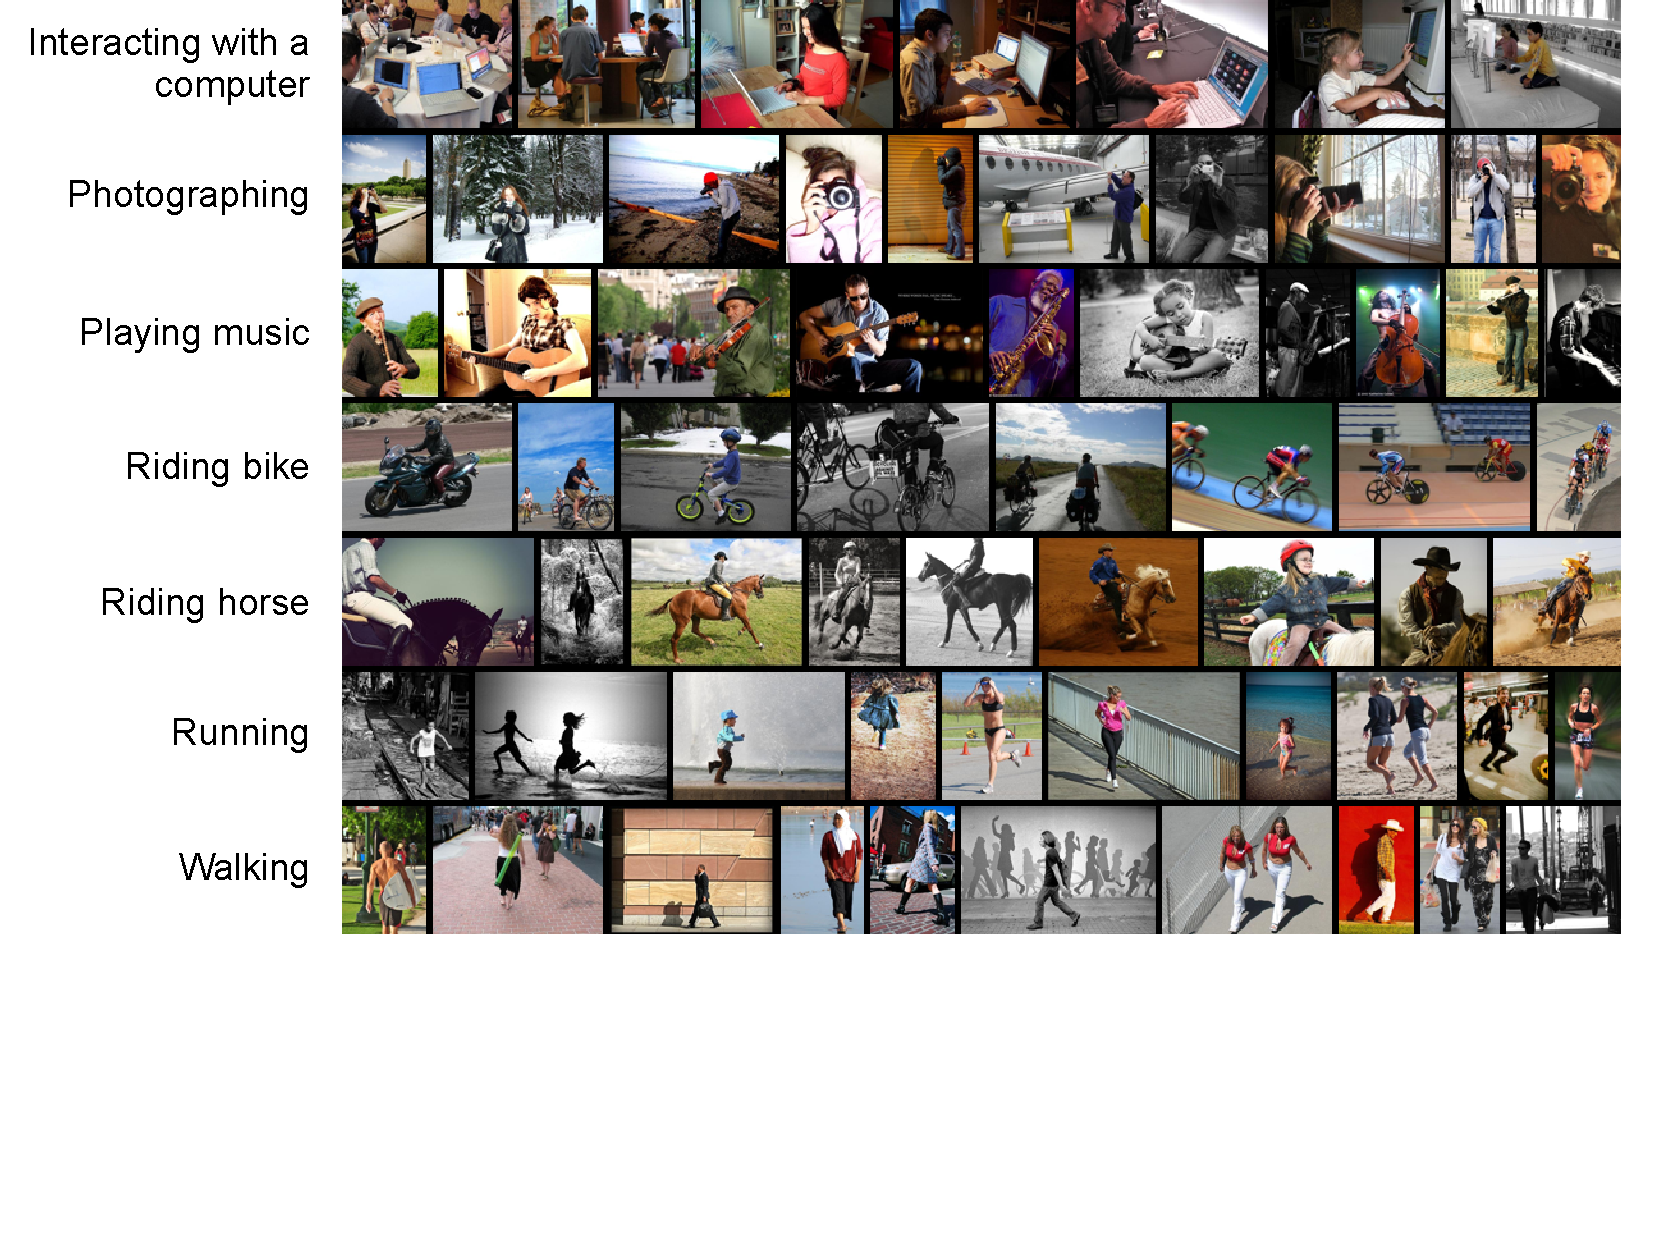
\includegraphics[width=1\linewidth]{figs/my_dataset_cropped.pdf}
\end{frame}

%------------------------------------------------------------------------------

\begin{frame}
\frametitle{Classification task}
Each person is annoted with a bounding box (smallest rectangle containing its visible pixels)
and the action being executed.

\vspace{0.3cm}
In the following, we are interessted in the 7-class classification problem.
The training set consists in 70 images of each type of action, so that at least 48 images
per class remain for test.

\vspace{0.3cm}
We mesure the performances using:
\begin{enumerate}[i]
\item {\em the classification accuracy}: average of the diagonal of the confusion table
\item {\em the mean average precision (mAP)}: mean area under the precision-recall curve of each 1-vs-all classifiers.
\end{enumerate}

\end{frame}

%------------------------------------------------------------------------------

%==============================================================================
\section{Bag-of-features classifier}

\begin{frame}
\frametitle{Bag-of-features classifier}
Here we investigate the influence of various type of parameters in the classifier
performances:

\begin{itemize}
\item \textbf{Image representation}: Images are represented using the spatial pyramid 
representation from Lazebnik~\etal~.
\item \textbf{SVM Classification}: We use 1-vs-all classification scheme. We investigate
the efficiency of different kernels.
\item \textbf{Using context information}: We analyse the impact of the context using
information provided by the bounding box.
\end{itemize}

\end{frame}

%------------------------------------------------------------------------------
\subsection{Image representation}

\begin{frame}
\frametitle{Bag-of-features classifier: Image representation}

\begin{itemize}
\item Features are extracted from multi-scale dense sampled SIFT descriptors.
\item Visual vocabulary is built from k-means clustering. Size of the dictionnary $K \in \{256, 512, 1024, 2048, 4096\}$.
\item Following Lazebnik~\etal~, we use a 2 levels spatial pyramid: image is divided into $1 \times 1$, $2 \times 2$ and $4 \times 4$
grids of cells leading to a $(1+4+16)K = 21K$ dimensional reprensation of an image.

\end{itemize}

\center
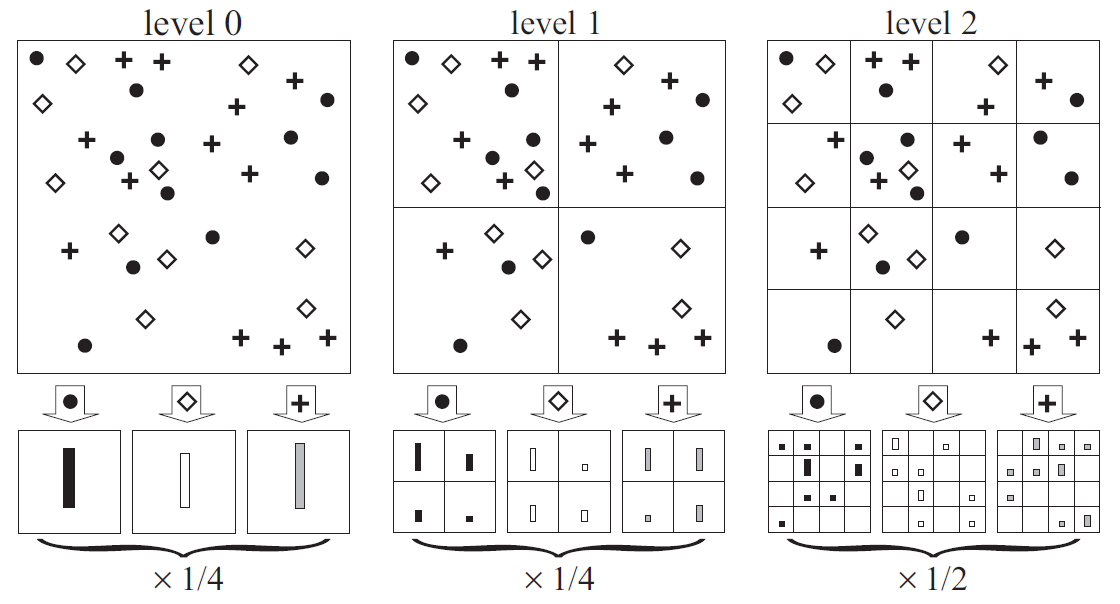
\includegraphics[width=0.5\linewidth]{figs/spatial_pyramid.png}

\end{frame}

%------------------------------------------------------------------------------

\subsection{SVM Classification}
\begin{frame}
\frametitle{Bag-of-features classifier: SVM Classification}

Classification is performed with
the SVM classifier using the 1-vs-all scheme, which, in our experiments, resulted in a small but consistent improvement
over the 1-vs-1 scheme. 
 
We investigate four different kernels: 
\begin{enumerate}
\item the histogram intersection kernel, given by $\sum_i \min(x_i,y_i)$;
\item the $\chi^2$ kernel, given by $\exp\{\frac{1}{\gamma} \sum_i \frac{(x_i-y_i)^2}{x_i+y_i}\}$; 
\item  the Radial basis function (RBF) kernel, given by  $\exp\{\frac{1}{\beta} \sum_i (x_i-y_i)^2\}$; and
\item the linear kernel given by $\sum_i x_i y_i$,
\end{enumerate}

where $\v x$ and $\v y$ denote visual word histograms of images $X$ and $Y$, and $\gamma$ and $\beta$ are
kernel parameters.

\end{frame}


%------------------------------------------------------------------------------ 

\subsection{Using context information}
\begin{frame}
\frametitle{Bag-of-features classifier: Using context information}

We consider the following four approaches:
\begin{enumerate}
\item[A.] {\bf ``Person"} 
\item[B.] {\bf ``Image"} 
\item[C1.] {\bf ``Person+Background''} 
\item[C2.] {\bf ``Person+Image''}
\end{enumerate}

\end{frame}


%==============================================================================
\section{Discriminatively trained part-based model}


%==============================================================================
\section{Experimental results}



\end{document}
